\documentclass[../stats.tex]{subfiles}
\graphicspath{{\subfix{../figures/}}}
\begin{document}
\chapter{Probability, Random Variables, and Probability Distributions}
\section{Basic Probability and Simulations}
What is Probability?
\begin{itemize}
    \item Outcomes are governed by chance, but in many repetitions a pattern emerges.
    \item Sample Space: all of the possible outcomes 
    \item Event: a specific, desired outcome or set of outcomes 
    \item Notation: probability of Event A $\rightarrow$ P(A)
    \item Range of Probabilities: the probability of an event is between 0 and 1 
    \item Sum of Probabilities: the probability of the whole sample is 1
\end{itemize}

Theoretical Probability - What should happen given the sample space.

This is the desired outcomes divided by the total outcomes.

Empirical Probability - When you are performing a simulation or experiment, it is what does happen given the trials.

This is the number of successes divided by trials.

The law of large numbers states that simulated (empirical) probabilities tend to get closer to the true (theoretical probability) as the number of trials increases.

\begin{center}
    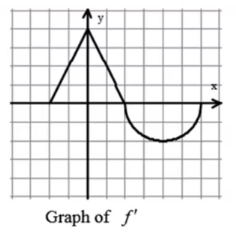
\includegraphics[width=0.8\textwidth]{4.1.1.PNG}
\end{center}
Probability can be written in the forms of fractions, decimals, or percentages.

For our class, we will write probabilities as decimals, rounded to four decimal places.

\begin{example}
    A bag contains 10 marbles - 2 black, 3 blue, 1 red, and 4 white.

    (a) What is the probability you will pull out a white marble?

    P(White) = 4/10 = 0.40

    (b) What is the probability you will pull out a blue marble?

    P(Blue) = 3/10 = 0.30
\end{example}

\begin{example}
    In the spinner below, each wedge is equal in area.
    \begin{center}
        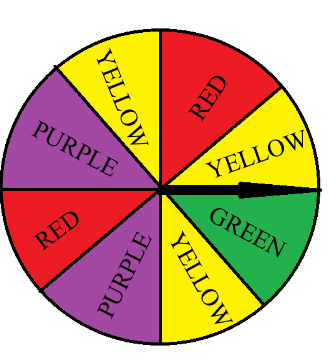
\includegraphics[width=0.8\textwidth]{4.1.2.PNG}
    \end{center}

    (a) What is the probability that the spinner will land on a red wedge?

    P(red) = 2/8 = 0.25 

    (b) What is the probability that the spinner will land on a yellow wedge?

    P(yellow) = 3/8 = 0.375
\end{example}

The notation for the probability that an event does not occur is P(A$^c$). We also refer to this as ``Not A'' in words.

The probability that an event does not occur is P(A$^c$) = 1-P(A).

Sometimes, it is easier to compute the complement of an event, than the event itself.

\begin{example}
    A coin is flipped three times and the results of each flip is noted.

    (a) Draw a sample space for this event.
    \begin{center}
        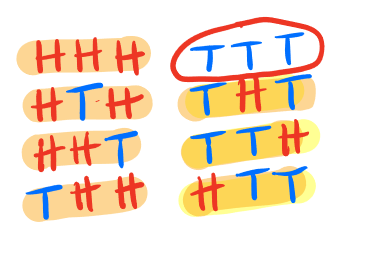
\includegraphics[width=0.8\textwidth]{4.1.3.PNG}
    \end{center}

    (b) What is the probability a series of three flips will produce exactly one head?

    P(1 head) = 3/8 = 0.375

    (c) What is the probability that a series of three flips will produce at least one head?

    P(at least 1 Head) = 1 - P(no Heads) = 7/8 = 0.875
\end{example}

Myth of ``Law of Averages''
\begin{itemize}
    \item The idea of probability is that randomness is predictable in the long run.
    \item Probability does not allow us to make short run predictions.
    \item Probability tells us random behavior evens out in the long run.
    \item Future outcomes are not affected by past behavior.
\end{itemize}

\begin{example}
    A group of 50 high school students were interviewed and asked what their favorite leisure activity is. Use the results in the table below to find and interpret the following probabilities.
    \begin{center}
        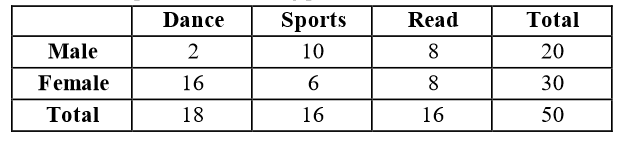
\includegraphics[width=0.8\textwidth]{4.1.5.PNG}
    \end{center}

    (a) What is the probability of picking a male whose favorite leisure activity is dance?

    P(male and dance) = 2/50 = 0.04

    (b) What is the probability of picking a person whose favorite leisure activity is reading?

    P(reading) = 0.32

    (c) What is the probability of picking someone who does not consider dance as their favorite leisure activity?

    P(not dance) = 1 - P(dance) = 0.64

    (d) Given that you've selected a female, what is the probability she likes reading?

    P(read | female) = 8/30 = 0.2667
\end{example}

The imitation of chance behavior, based on a model that accurately reflects the situation, is called a simulation. Simulations are usually done with a table of random digits, random number generator, dice, deck of cards, spinner, etc.

Four Principles of Simulation:

State - Identify the probability calculation.

Must include:
\begin{itemize}
    \item Identify variable.
    \item Statement of probability in symbols or words.
\end{itemize}

Plan - Describe how to use your chance process.

Must include:
\begin{itemize}
    \item What tool?
    \item What values are you assigning?
    \item How many values are you picking each time?
    \item How many times do you run the simulation?
    \item What about repeat digits or ignored digits?
    \item What are you recording?
\end{itemize}

Do - Perform the simulation (trials typically indicated, perform at least 10 if not).

Must include:
\begin{itemize}
    \item Simulation data, if number of trials is 10 or less.
    \item Summary of data for larger trials.
\end{itemize}

Conclude - Use the results of your simulation to answer the question.

Must include:
\begin{itemize}
    \item Statement of probability.
    \item Answer to question.
    \item Usually about being surprised/reasonable/expected, etc.
\end{itemize}

\begin{example}
    What is the probability that a student gets 6 out of 6 questions correct on a true/false quiz written in Greek? (Assume the exam taker does not know any Greek.) Should the instructor be concerned about cheating? Perform a simulation to answer this question.

    \begin{itemize}
        \item What is the probability of guessing 6/6 correct on a T/F quiz?
        50\% correct or 50\% incorrect 
        \item Label digits 0-4 as correct and 5-9 as incorrect. Using a random digit table, select 1 number at a time (repeats allowed) and record if correct or incorrect. Perform this simulation 6 times to represent one quiz. Count how many questions are ``correct''. Repeat for 20 trials.
    \end{itemize}
    \begin{center}
        \begin{tabular}{c|c}
            \# Correct & \# Trials \\\hline 
            0 & 0\\
            1&2\\
            2&3\\
            3&8\\
            4&5\\
            5&2\\
            6&0
        \end{tabular}
    \end{center}
    After conducting the simulation, we see that we had no trials where 6/6 is correct by guessing. We should be suspicious of the result the student got.
\end{example}

\section{The Addition Rule}
Mutually Exclusive Events 
\begin{itemize}
    \item When two events have no outcomes in common, we refer to them as mutually exclusive events.
    \item P(A and B) = 0
    \item P(A or B) = P(A) + P(B)
\end{itemize}

\begin{example}
    Let's revisit our ``rolling the dice'' game, where the italicized numbers represent the sum of the dice rolled.
    \begin{center}
        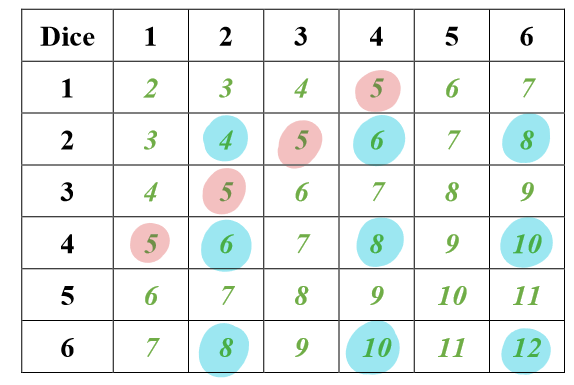
\includegraphics[width=0.8\textwidth]{4.2.1.PNG}
    \end{center}
    Let A be rolling a sum of 5 and B be rolling two even numbers.

    These events are mutually exclusive because they have no outcomes in common.

    P(A) is 4/36, and P(B) is 9/36, so P(A or B) is 13/36.    
\end{example}

\begin{example}
    Identify if the following events are mutually exclusive. If they are not, given an example of where they overlap.

    (a) Rolling a sum of 4 and rolling doubles.

    Not mutually exclusive. Ex. 2, 2

    (b) Rolling an odd sum and rolling a 3.

    Not mutually exclusive. Ex. 3, 4

    (c) Rolling a 4 and rolling a sum of 12

    Mutually exclusive

    (d) Rolling an odd number and rolling a sum of 10 

    Not mutually exclusive. Ex. 5, 5
\end{example}

\begin{example}
    Find the probability of rolling doubles or a sum of 8.
    \begin{center}
        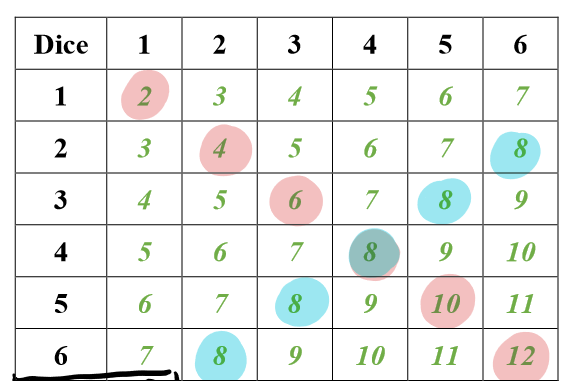
\includegraphics[width=0.8\textwidth]{4.2.2.PNG}
    \end{center}

    Let A be rolling doubles, and B be rolling a sum of 8.

    They are not mutually exclusive events.

    P(A) = 6/36 and P(B) = 5/36. We have to subtract P(A and B) = 1/36 from this, and we get P(A or B) = 10/36.
\end{example}

If A and B are any two events resulting from some chance process, then 
\begin{center}
    P(A or B) = P(A) + P(B) - P(A and B)
\end{center}
Notice how if A and B are mutually exclusive, P(A and B) = 0 and P(A or B) = P(A) + P(B) - 0

How do we know the value of P(A and B)? For now, we will use common sense and drawing out the sample space, but the general multiplication rule will allow us to find this mathematically later.

\begin{example}
    A card is selected at random from a deck of 52 cards. Determine if the following events are mutually exclusive and then find the probability of the events.
    \begin{center}
        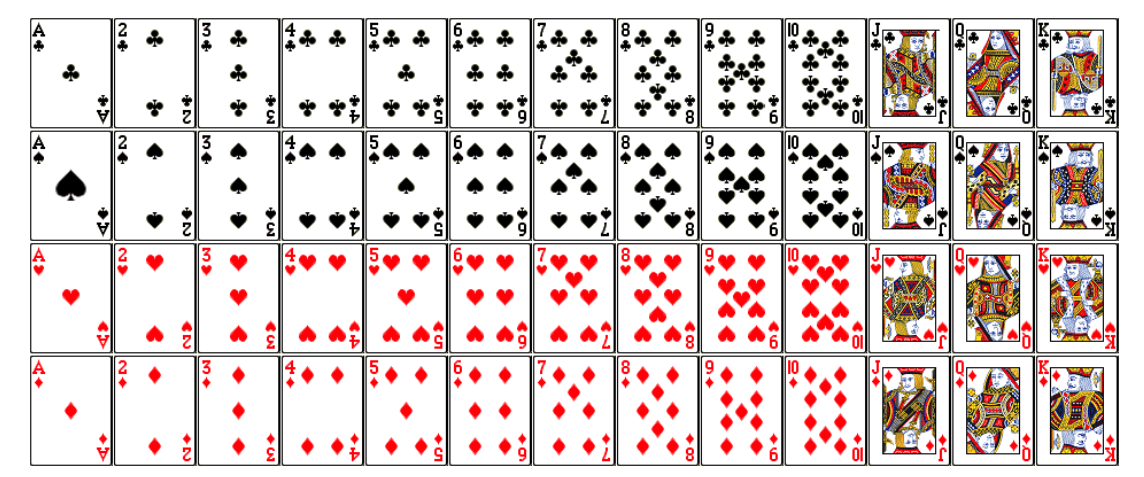
\includegraphics[width=0.8\textwidth]{4.2.3.PNG}
    \end{center}

    (a) P(red or Queen) 

    Not mutually exclusive. 26/52 + 4/52 - 2/52 = 28/52.

    (b) P(Ace or King)

    Mutually exclusive. 4/52 + 4/52 = 8/52

    (c) P(Queen or even)

    Mutually exclusive. 4/52 + 20/52 = 24/52 

    (d) P(black or odd)

    Not mutually exclusive. 26/52 + 16/52 - 8/52 = 34/52
\end{example}

\begin{example}
    You were interested in how many students at your school regularly eat breakfast. You conducted a survey, asking, ``Do you eat breakfast on a regular basis?'' Your random sample consisted of 600 students at the school and the results are shown in the table below.
    \begin{center}
        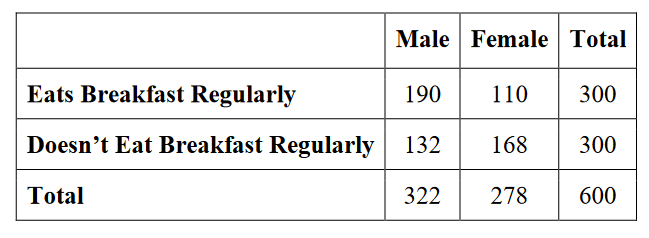
\includegraphics[width=0.8\textwidth]{4.2.4.PNG}
    \end{center}

    If we select a student from this sample at random, what is the probability that the student is

    (a) A female?

    P(female) = 278/600

    (b) Someone who eats breakfast regularly?

    P(Breakfast) = 300/600

    (c) A female and eats breakfast regularly?

    P(female and breakfast) = 110/600

    (d) A female or east breakfast reguarly?

    P(female or breakfast)

    278/600 + 300/600 - 110/600 = 468/600
\end{example}


\section{Venn Diagrams and the Multiplication Rule}
Union and Intersection 
\begin{itemize}
    \item We can represent events with a Venn Diagram - a display of potential probabilities.
    \item The box around the Venn diagram represents the total sample space where P(S) = 1.
    \item The circles themselves represent the probability of each event.
\end{itemize}
\begin{center}
    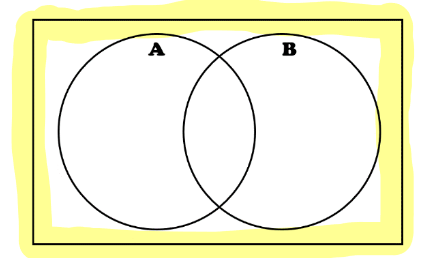
\includegraphics[width=0.8\textwidth]{4.3.1.PNG}
\end{center}

Union: OR = probability that either occurs. The symbol is $\cup$

Intersection: AND = probability both occur. The symbol is $\cap$
\begin{center}
    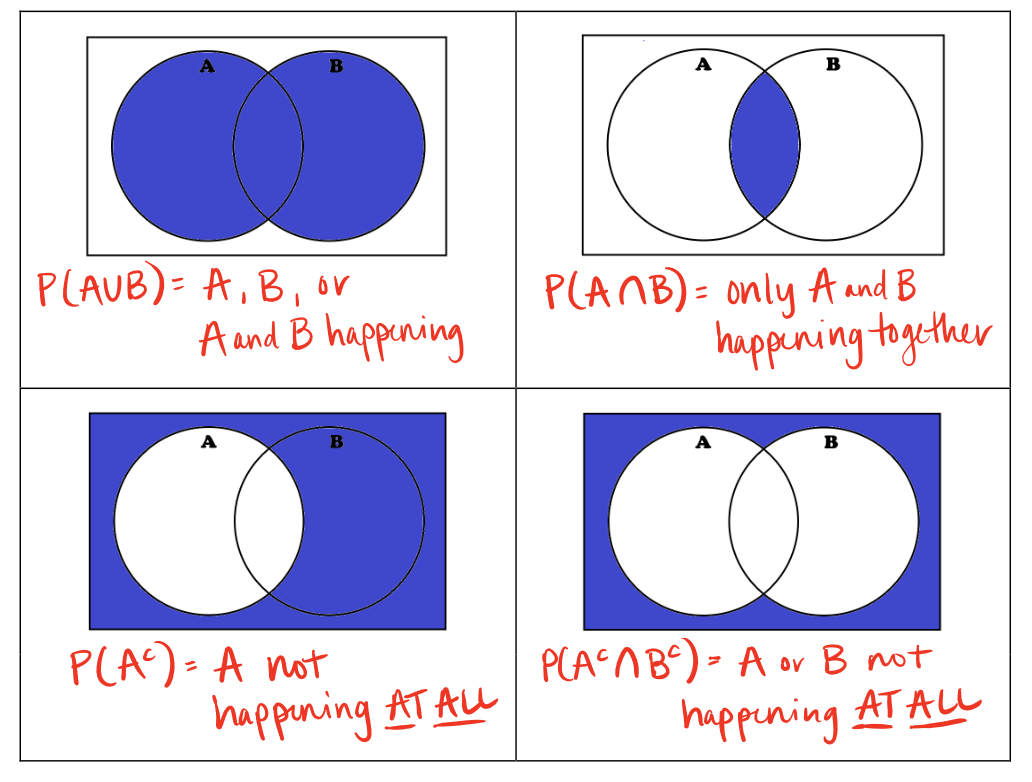
\includegraphics[width=0.8\textwidth]{4.3.2.PNG}
\end{center}

\begin{example}
    Shade the probabilities for the following notations.
    \begin{center}
        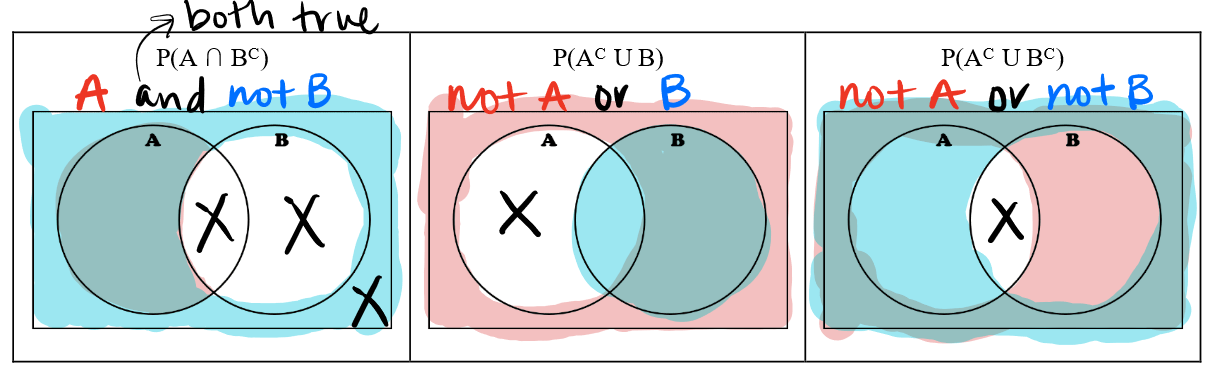
\includegraphics[width=0.8\textwidth]{4.3.3.PNG}
    \end{center}
\end{example}

\begin{example}
    In your statistics class, you are interested in exploring the taste preference of your classmates. You have two tastes, sweet and salty. 25 students were asked if they prefer both, only sweet, only salty, or neither. The following two-way table shows the data.
    \begin{center}
        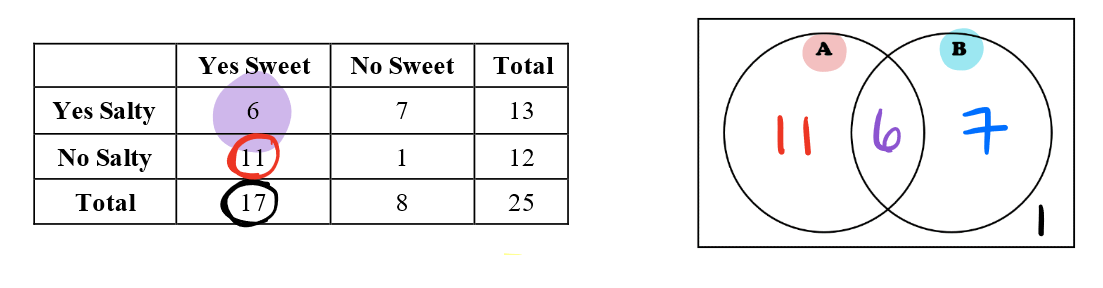
\includegraphics[width=0.8\textwidth]{4.3.4.PNG}
    \end{center}

    Let A = sweet and B = salty. Find and interpret the following probabilities.

    (a) P(A$\cap$B)

    6/25 = 0.24. The probability a student likes both salty and sweet foods is 24\%.

    (b) P(A$\cup$B)

    $\frac{11+6+7}{25}=0.96$. The probability a student likes either salty or sweet foods is 96\%.

    (c) P(A$\cap$B$^c$)

    $\frac{11}{25}=0.44$. The probability a student likes sweet but not salty foods is 44\%.

    (d) P(A$^c\cup$B)

    $\frac{7+1+6}{25}=0.56$. The probability a student likes no sweet foods or likes salty foods is 56\%.

    (e) P(A$\cup$B$^c$)

    $\frac{11+6+1}{25}=0.72$. The probability a student likes sweet foods or does not like salty foods is 72\%.

    (f) P(A$^c\cap$B$^c$)

    $\frac{1}{25}=0.04$. The probability a student does not like sweet foods and does not like salty foods is 4\%.
\end{example}

Multiplication rule for independent events
\begin{itemize}
    \item Two events are independent if they do not influence one another.
    \item The occurrence of one has no effect on the occurrence of the other.
    \begin{itemize}
        \item Toss a coin twice.
        \item The gender of each child born to the same mother.
        \item Trials with replacement.
    \end{itemize}
    \item If A and B are independent events, then the probability that both A and B occur is found using the multiplication rule.
\end{itemize}
\begin{center}
    P(A and B) = P(A$\cap$B) = P(A)$\cdot$P(B)
\end{center}

\begin{example}
    Find the probabilities.

    (a) I flip a coin and then roll a dice. What is the probability I flip a head and then roll a 5?

    $\left(\frac{1}{2}\right)\left(\frac{1}{6}\right) = 0.0833$

    (b) What is the probability that a mother will have 4 girls in a row?

    $\left(\frac{1}{2}\right)^4 = 0.0625$.

    (c) I have a standard deck of 52 cards. What is the probability I pull a red card, replace it and shuffle, and then pull a black card?

    $\left(\frac{1}{2}\right)\left(\frac{1}{2}\right) = 0.25$

    (d) You spin the following spinner 5 times. What is the probability you land on yellow all 5 times?
    \begin{center}
        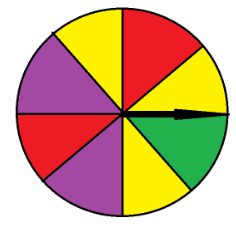
\includegraphics[width=0.8\textwidth]{4.3.5.PNG}
    \end{center}

    $\left(\frac{3}{8}\right)^5 = 0.0074$.
\end{example}

Multiplication Rule for Dependent Events 
\begin{itemize}
    \item Two events are dependent if they influence one another.
    \item The occurrence of one affects the occurrence of the other.
    \begin{itemize}
        \item Trials without replacement.
    \end{itemize}
    \item If A and B are dependent events, then the probability that both A and B occur is found using:
\end{itemize}
\begin{center}
    P(A and B) = P(A$\cap$B) = P(A)$\cdot$P(B$|$A)
\end{center}
\begin{itemize}
    \item Where P(B$|$A) is the probability of B ``given'' that A has occurred.
    \item The conditional probability of an event is the probability that one event will happen, if it is known that another event has happened.
\end{itemize}

\begin{example}
    Find the probabilities.

    (a) I have a standard deck of 52 cards. What is the probability of pulling a spade and then a 5?

    $\left(\frac{13}{52}\right)\left(\frac{4}{51}\right) = 0.0196$

    (b) I have a standard deck of 52 cards. What is the probability of pulling a jack and then another jack?

    $\left(\frac{4}{52}\right)\left(\frac{3}{51}\right) = 0.0045$

    (c) In your statistics class, you are interested in exploring the taste preference of your classmates. You have two tastes, sweet and salty. 25 students were asked if they prefer both, only sweet, only salty, or neither. The following two-way table shows the data.
    \begin{center}
        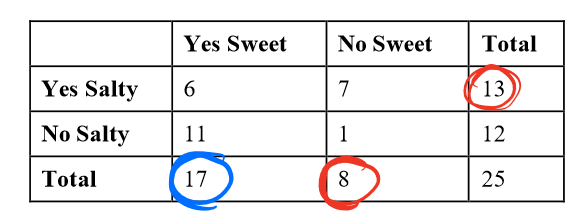
\includegraphics[width=0.8\textwidth]{4.3.6.PNG}
    \end{center}

    What is the probability you select someone who likes salty food then select another person who likes salty food?

    $\left(\frac{13}{25}\right)\left(\frac{12}{24}\right) = 0.26$

    What is the probability you select someone who does not like sweet food then select a person who likes sweet food?

    $\left(\frac{8}{25}\right)\left(\frac{17}{24}\right) = 0.2267$
\end{example}

\section{Conditional Probability and Tree Diagrams}
Rule for conditional probability:
\begin{itemize}
    \item If A and B are dependent events, then the probability that both A and B occur is found using P(A$\cup$B) = P(A)$\cdot$P(B$|$A) where P(B$|$A) is the probability of B ``given'' that A has already occurred
    \item The conditional probability of an event is the probability that one event will happen, if it is known that another event has happened.
    \item We can rearrange the multiplication rule a little and get a formula for conditional probability:
\end{itemize}
\begin{center}
    P(B$|$A) = $\frac{P(A\cap B)}{P(A)}$
\end{center}

Why does this formula make sense?
\begin{itemize}
    \item When you know something has happened, it changes the sample space - specifically, it shrinks to the given event.
    \item If we know A has already occurred, that becomes your ``sample space''.
    \item Then, for B to occur, it has to occur with A, which is the intersection of A and B.
\end{itemize}
\begin{center}
    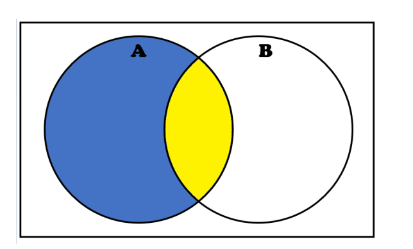
\includegraphics[width=0.8\textwidth]{4.4.1.PNG}
\end{center}

\begin{example}
    Use the two-way table below to calculate the indicated probabilities.
    \begin{center}
        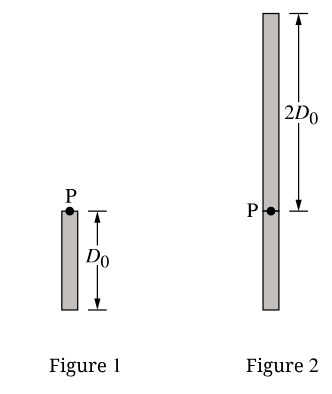
\includegraphics[width=0.8\textwidth]{4.4.2.PNG}
    \end{center}

    (a) If we select a women and find she has brown hair, what is the probability that she will also have hazel eyes?

    P(Hazel Eyes$|$Brown Hair) = $\frac{P(HE\cap BH)}{P(BH)} = \frac{29/313}{143/313}= 0.2028$

    (b) If we select a woman and find she has brown eyes, what is the probability that she will also have black hair?

    P(Black Hair$|$Brown Eyes) = $\frac{P(BH\cap BE)}{P(BE)} = \frac{36}{122} = 0.2951$
\end{example}

Showing Independence:
\begin{itemize}
    \item If we draw two cards with replacement, we know that those events are independent.
    \item If we draw two cards without replacement, we know that those events are dependent.
\end{itemize}

However, in the real world, it can be difficult to determine if two events are independent or dependent. We do have a way to prove independence, however, using either of the following formulas.
\begin{center}
    P(A$\cap$B) = P(A)$\cdot$P(B) or P(A) = P(A$|$B)
\end{center}

\begin{example}
    Below is a two-way table that shows produce and how many packages are purchased based on whether it is fresh or frozen.
    \begin{center}
        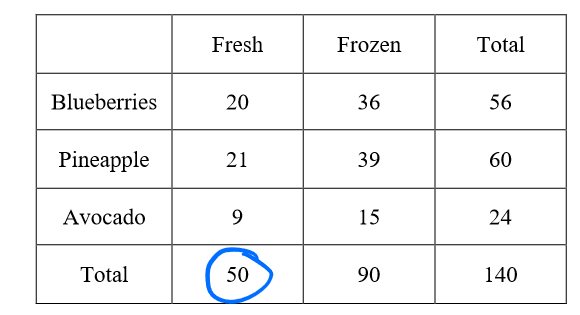
\includegraphics[width=0.8\textwidth]{4.4.3.PNG}
    \end{center}

    (a) Are ``blueberries'' and ``fresh'' independent?

    P(B) = P(B$|$Fresh), 0.4=0.4, so independent.

    (b) Are ``avocados'' and ``frozen'' independent?

    P(Frozen$\cap$Avocados) = P(Frozen)$\cdot$P(A), and $\frac{15}{140}\neq \frac{90}{140}\cdot\frac{24}{140}$. They are not independent.
\end{example}

Tree Diagrams
\begin{example}
    A company manufacturing electronic components for home entertainment systems buys electrical connectors from three suppliers. The company prefers to use supplier A because only 
    2\% of those connectors prove to be defective, but supplier A can deliver only 55\% of the connectors needed. The company must also purchase connectors from two other suppliers, 40\% from supplier B and the rest from supplier C. The rates of defective connectors from B and C are 4\% and 5\%, respectively. You buy one of these components.
    \begin{center}
        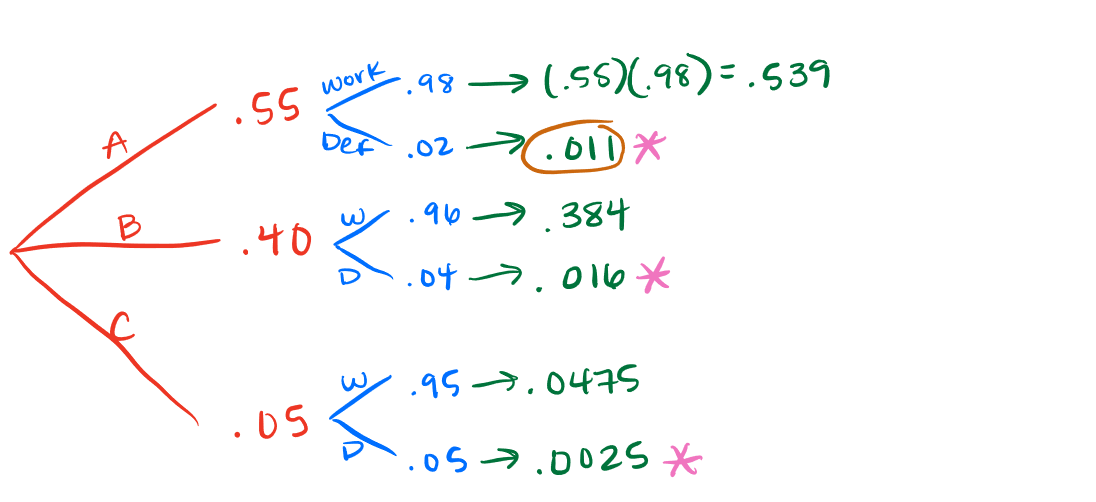
\includegraphics[width=0.8\textwidth]{4.4.4.PNG}
    \end{center}

    (a) What is the probability that you use supplier B to and the connector is defective?
    
    P(B$\cap$Defective) = $(0.40)(0.04)=0.016$

    (b) What's the probability that you find that the connector is defective?

    P(Defective) = $0.011+0.016+0.0025=0.0295$

    (c) Given that the component is defective, what is the probability it came from supplier A?

    P(A$|$Defective) = $\frac{P(A\cap \text{defective})}{P(\text{defective})} = \frac{0.011}{0.0295}=0.3729$
\end{example}

\begin{example}
    The probability that a person has a particular virus is 1 out of 250. If they have the virus, the probability they test positive for the virus is 0.90. If they do not have the virus, the probability they test positive for the virus is 0.15.
    \begin{center}
        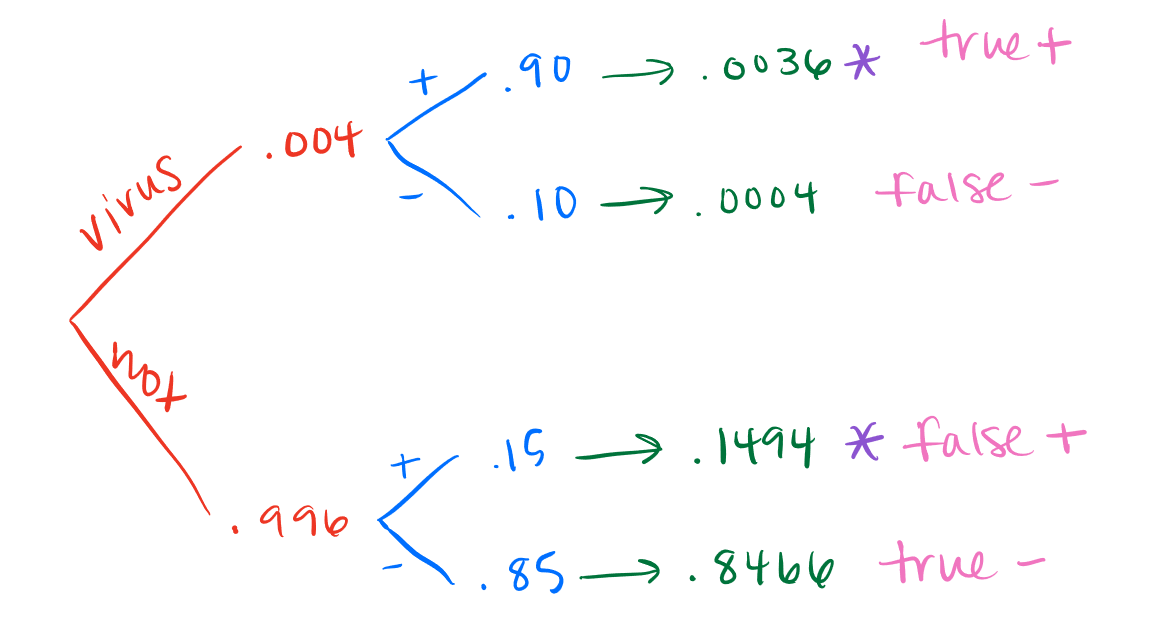
\includegraphics[width=0.8\textwidth]{4.4.5.PNG}
    \end{center}

    (a) Given that a person tests positive for the virus, what is the probability they have the virus?

    P(virus$|$+) = $\frac{P(\text{virus}\cap +)}{P(+)} = \frac{0.0036}{0.0036+0.1494}=0.0235$

    (b) What is the probability of a person testing and getting a false positive?

    P(false+) = P(no virus$\cap$ +) = 0.1494
\end{example}


\section{Discrete and Continuous Random Variables}
A random variable takes numerical values that describe the outcomes of some chance process. Random variables involve the same probability rules we have already learned, but we will extend those rules to be able to model more events.

\begin{example}
    Suppose we toss a coin 3 times.

    This is the sample space.
    \begin{center}
        
\includegraphics[width=0.8\textwidth]{4.5.1.PNG}
    \end{center}
    The total number of outcomes is 8, the probability of any one outcome is 1/8.

    Let X be the number of heads out of 3 coin tosses.
    \begin{center}
        \begin{tabular}{c|c|c}
            Symbols & Meaning & Probability \\\hline 
            X = 0& no heads out of 3 tosses & 1/8\\\hline
            X = 1& 1 heads out of 3 tosses & 3/8\\\hline
            X = 2& 2 heads out of 3 tosses & 3/8\\\hline
            X = 3& 3 heads out of 3 tosses & 1/8
        \end{tabular}
    \end{center}
    With these 4 X values, and their corresponding probabilities, we can create a frequency table and a histogram to describe this event.
    \begin{center}
        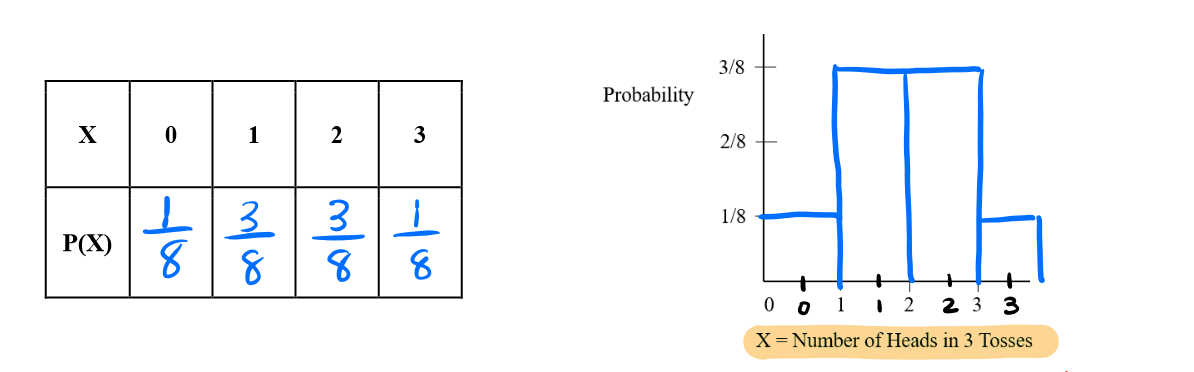
\includegraphics[width=0.8\textwidth]{4.5.2.PNG}
    \end{center}

    \begin{itemize}
        \item The frequency table and histogram above each represent a probability distribution.
        \item A probability distributions tells us the value that our random variable can take and the probability associated with each value.
    \end{itemize}
\end{example}

Every probability distribution must satisfy each of the following requirements.
\begin{enumerate}
    \item There is a numerical (not categorical) random variable X, and each of the values of X has an associated probability with it.
    \item The sum of all the probabilities in the distribution $\sum P(X)$ must equal 1.
    \item $0\leq P(X)\leq 1$ for all probabilities in the distribution.
\end{enumerate}

Notation:
\begin{center}
    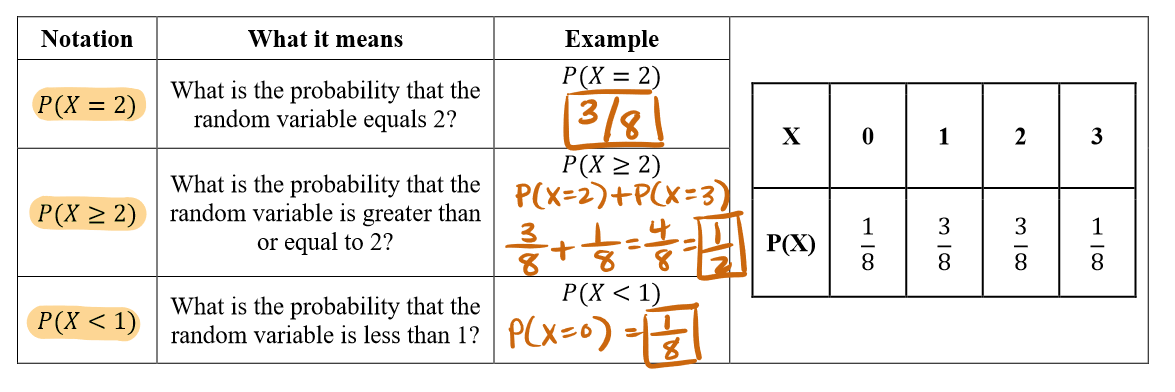
\includegraphics[width=0.8\textwidth]{4.5.3.PNG}
\end{center}

A discrete random variable takes on a fixed set of possible values with whole number outcomes.
\begin{itemize}
    \item Random variables are usually capital letters (X, Y, Z, etc.)
    \item Random variables can be discrete or continuous (continuous is next lesson)
    \item Random variables must be numeric in value.
    \begin{itemize}
        \item In our example, even though a result of Head or Tails is categorical, we described it numerically.
    \end{itemize}
\end{itemize}

The mean of a discrete random variable X, is the mean outcome for infinitely many trials.

We think of this as the ``expected value'' because it is the average value we would expect to get if the trials could continue indefinitely. (Not what we expect to get in a single trial)

To find the mean, $\mu_x$, or expected value, $\sum(x)$, of a discrete random variable X, multiply each possible value by its probability, then add all the products.
\begin{center}
    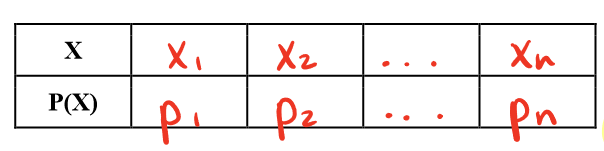
\includegraphics[width=0.8\textwidth]{4.5.4.PNG}
\end{center}
\[ mu_x = x_1\cdot p_1+x_2\cdot p_2+\dots x_n\cdot p_n = E(x) = \sum x_i\cdot p_i \]
\begin{example}
    Northwestern University posts the grade distributions for its courses online. Students in Statistics 101 in a recent semester received 26\% A's, 42\% B's, 20\% C's, 10\% D's, and 2\% F's.

    (a) Create a probability distribution for the random variable X, which represents the student's grade on a four point scale (with A = 4)
    \begin{center}
        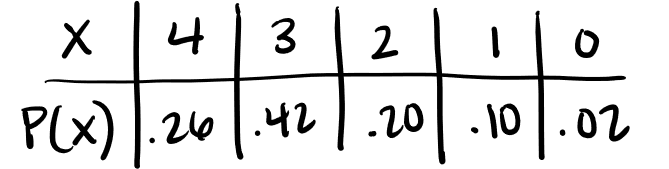
\includegraphics[width=0.8\textwidth]{4.5.5.PNG}
    \end{center}

    (b) Find and interpret $P(X\geq 3)$ if X represents a randomly selected Statistics 101 student.

    P(X$\geq 3$) = P(X=3)+P(X=4) = 0.68. The probability that a randomly selected Stats 101 student gets a grade of A or B is 68\%.

    (c) Write the event ``the student got a grade worse than C'' in terms of values of the random variable X. What is the probability of this event?

    P($x<2$) = P(x=1) + P(x=2) = 0.10 + 0.02 = 0.12

    (d) Compute the mean of the random variable X. Interpret this value in context.

    $\mu_x = (4)(0.26)+(3)(0.42)+(2)(0.20)+(1)(0.10)+(0)(0.02) = 2.8$. If many students took this course, we would expect an average grade of 2.8, which is between a B and C.
\end{example}

The standard deviation of a random variable X is a measure of how much the values of the variable typically vary from the expected value.
\begin{center}
    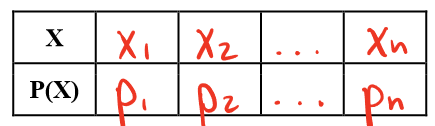
\includegraphics[width=0.8\textwidth]{4.5.6.PNG}
\end{center}
\[ \sigma_x^2 = (x_1-\mu_x)^2\cdot p_1+(x_2-\mu_x)^2\cdot p_2+\dots + (x_n-\mu_x)^2\cdot p_n \]
\[ \sigma_x^2 = Var(X)=\sum(x_1-\mu_x)^2\cdot p_i \]
\[ \sigma_x = \sqrt{\sum (x_i-\mu_x)^2\cdot p_i}\]

\begin{example}
    For the Northwestern example, find and interpret the standard deviation of the grade probability distribution.

    $\sigma_x = \sqrt{(4-2.8)^2(.26)+(3-2.8)^2(.42)+(2-2.8)^2(.2)+(1-2.8)^2(.1)+(0-2.8)^2(.02)}=1$

    If many students took this course, we would expect the typical deviation from the mean to be about 1 letter grade.
\end{example}

Continuous Random Variable 
\begin{itemize}
    \item Continuous Random Variables take on all possible values in an interval of numbers. The probability distribution of X is described by a density curve.
    \item The probability of any event is the area under the density curve and above, below, or between the values x that define the event.
    \item Area under a density curve is always equal to 1.
    \item The probability is on the $y$-axis in a distribution, so finding the area equates to finding the probability of getting an interval of numbers.
    \item The probability at an event is 0 for a continuous random variable because the area under a point is 0.
    \item The mean and standard deviation of a continuous random variable are found using integration, so we will not discuss their formulas here.
\end{itemize}

Continuous random variables are usually represented as functions in practice. The continuous random variable we will explore is the normal distribution, and we will revisit it at the start of Unit 5.

Why do we have random variables?

This is an important question to keep in mind as we continue to look at different random variables. We need random variables because they represent more things than a single measurement can. One-variable statistics used data, where random variables can use theory and apply it to real situations.

Calculator: Mean and Standard Deviation from a Probability Distribution Table 
\begin{itemize}
    \item Enter outcomes into L1 and probabilities into L2 
    \item Run 2nd - VARS - 1VarStats with List:L1 and FreqList:L2 
    \item Mean will be represented by $\overline{x}$
    \item Standard deviation will be represented by $\sigma_x$
\end{itemize}

\section{Combining Random Variables}
\begin{example}
    Let X and Y be two independent variables with the following probability distribution.
    \begin{center}
        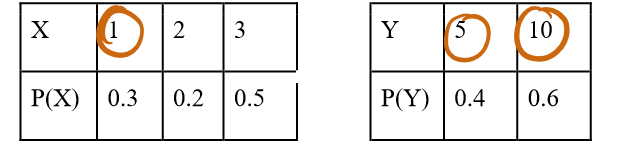
\includegraphics[width=0.8\textwidth]{4.6.1.PNG}
    \end{center}
    If we let S = X + Y, create the probability distribution below.
    \begin{center}
        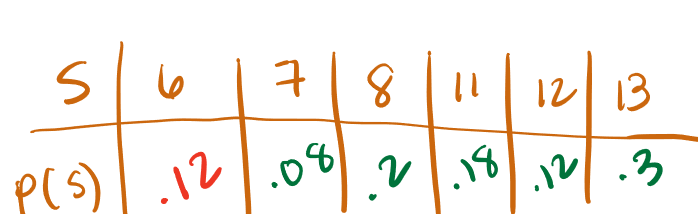
\includegraphics[width=0.8\textwidth]{4.6.2.PNG}
    \end{center}

    Now we can find the following:
    \begin{itemize}
        \item E(S) = 10.2 
        \item E(X) = 2.2
        \item E(Y) = 8
        \item $\sigma_S = 2.6$
        \item $\sigma_X = 0.87$
        \item $\sigma_Y = 2.45$
    \end{itemize}
\end{example}

There is a shortcut for finding means and standard deviations of combined random variables without having to create a new distribution!

If X and Y are two independent random variables:
\[ E(X+Y)=E(X)+E(Y)\]
\[ E(X-Y)=E(X)-E(Y)\]
\[ \sigma_{X+Y}=\sigma_{X-Y}=\sqrt{\sigma_X^2+\sigma_Y^2}\]

With the problem above, if you insert the values, you can see that they are the same.

\begin{example}
    The head folks at Google decided to try a random salary assignment for their workers this year!
    They have the following probability distribution, where X = salary.
    \begin{center}
        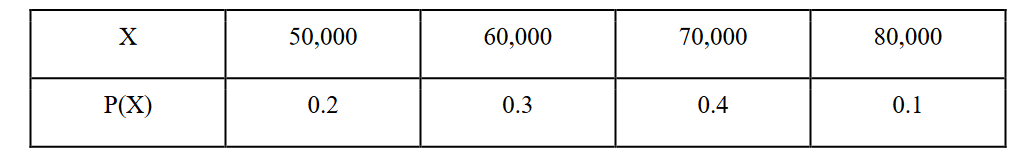
\includegraphics[width=0.8\textwidth]{4.6.3.PNG}
    \end{center}

    (a) What is the expected salary for a Google employee? What is the standard deviation?

    $\mu_x=\$64,000$, $\sigma_x = \$9165.15$

    (b) Google decides to give everyone a \$500 bonus. Create a new probability distribution and find the expected value and standard deviation. Notice anything?
    \begin{center}
        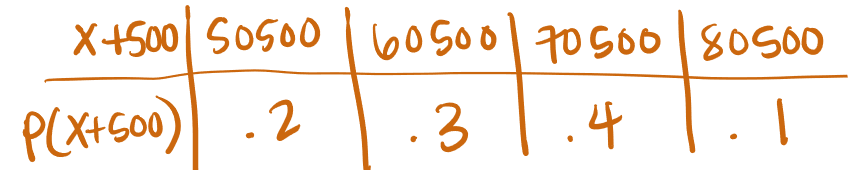
\includegraphics[width=0.8\textwidth]{4.6.4.PNG}
    \end{center}
    The expected value increased by \$500, but the standard deviation remained the same.

    (c) Google decides that it will pay cash at the end of the year for this salary. They will give out \$100 bills. Let X = number of \$100 bills they will give out. Create a new 
    probability distribution (use the bonus distribution) and find the expected value and standard deviation. Notice anything?
    \begin{center}
        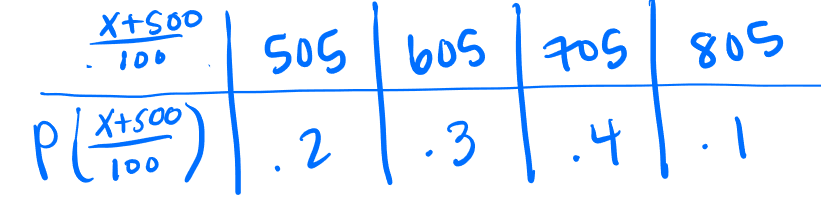
\includegraphics[width=0.8\textwidth]{4.6.5.PNG}
    \end{center}
    In this case, both the mean and standard deviation were divided by 100.
\end{example}

If X is a random variable and a and b are both constants:
\[ E(a+bX)=a+bE(X)\]
\[ \sigma_{a+bX}=|b|E(x)\]

\begin{example}
    For an upcoming concert, each customer may purchase up to 3 child tickets and 3 adult tickets. Let C be the number of child tickets purchased by a single customer. The probability distribution of the number of child tickets purchased by a single customer is given in the table below.
    \begin{center}
        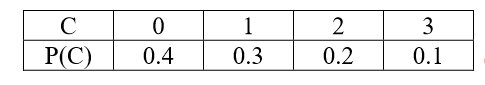
\includegraphics[width=0.8\textwidth]{4.6.7.PNG}
    \end{center}

    (a) Compute the mean and the standard deviation of C.

    $\mu_C$ = 1 child ticket, $\sigma_C$ = 1 child ticket.

    (b) Suppose the mean and the standard deviation for the number of adult tickets purchased by a single customer are 2 and 1.2, respectively. Assume that the number of child tickets and adult tickets purchased are independent random variables.
    Compute the mean and the standard deviation of the total number of adult and child tickets purchased by a single customer.

    $\mu_A = 2$, $\sigma_A=1.2$. 

    $T=A+C$, $\mu_T=\mu_A+\mu_C=3$ tickets.

    $\sigma_T=\sqrt{\sigma_A^2 + \sigma_C^2}=\sqrt{(1.2)^2+(1)^2}=1.562$ tickets.

    (c) Suppose each child ticket costs \$15 and each adult ticket costs \$25. Compute the mean and the standard deviation of the total amount per purchase.

    S = 25A = 15C, 
    
    $\mu_S = 25\mu_A+15\mu_C = \$65$

    $\sigma_S=\sqrt{(25\cdot\sigma_A)^2+(15\cdot\sigma_C)^2}=\$33.54$
\end{example}

\begin{example}
    Each full carton of Grade A eggs consists of 1 randomly selected empty cardboard container and 12 randomly selected eggs. The weights of such full cartons are approximately normally distributed with a mean of 840 grams and a standard deviation of 7.9 grams.

    The weights of the empty cardboard containers have a mean of 20 grams and a standard deviation of 1.7 grams. It is reasonable to assume independence between the weights of the empty cardboard containers and the weights of the eggs. It is also reasonable to assume independence among the weights of the 12 eggs that are randomly selected for a full carton.

    Let the random variable X be the weight of a single randomly selected Grade A egg.

    (a) What is the mean of X?

    1 container + 12 eggs, full carton has $\mu=840$, $\sigma=7.9$, empty container has $\mu=20$, $\sigma=1.7$

    $840=20+x_1+\dots+x_{12}$ so, $840=20+12X$, or $X=68.33$ grams.

    (b) What is the standard deviation of X?

    $7.9=\sqrt{(1.7)^2+\sigma_{x1}^2+\dots+\sigma_{x12}^2} \implies 62.41 = (1.7)^2+12\sigma_x^2$.

    Solving for $\sigma_x$ gives 2.227 grams.
\end{example}

\section{The Binomial Distribution}
Bernoulli Trials:

Requirements for a Bernoulli Trial:
\begin{enumerate}
    \item Two Possible Outcomes 
    \item Probability of Success is the Same for Each Trial 
    \item Trials are Independent
\end{enumerate}

If we take a Bernoulli Trial and then we are interested in the number of successes in a specific number of trials, we create a Binomial Probability Distribution.

There are four requirements for a setting to follow the binomial probability distribution. As long as these four things are true, we can use the binomial probability model for calculating the probabilities.
\begin{itemize}
    \item Binary:
    \begin{itemize}
        \item Each trial falls into one of two categories - we call them ``success'' or ``failure''.
        \item Success does not necessarily mean a positive outcome, but instead, the outcome we are looking for.
    \end{itemize}
    \item Independent Trials
    \begin{itemize}
        \item Each trial is independent of the next.
        \item Reasonable Assumption for coins, cards with replacement, spinners, rolling a die, etc.
        \item What about sampling without replacement, when it can't be avoided? This is where the ``10\% condition'' comes in.
        \begin{itemize}
            \item The 10\% condition says that if you are sampling from a large enough population, you can proceed with sampling without explacement as though the trials were independent.
            \item Ex. Sampling from a deck of cards without replacement would violate this but sampling people from a large town would be okay.
        \end{itemize}
    \end{itemize}
    \item Number of Trials is Fixed 
    \begin{itemize}
        \item We are counting the number of successes from a set number of trials (called n).
    \end{itemize}
    \item Same Probability
    \begin{itemize}
        \item The probability of success (called p) is the same for each trial.
    \end{itemize}
\end{itemize}

If all four points are satisfied, you can compute the probability you get a certain number of successes in a specified number of trials:
\[ P(X=x)=\binom{n}{x}p^x(1-p^{n-x})\] 
where $\binom{n}{x}=nC_x=\frac{n!}{x!(n-x)!}$. (MATH - PROB - 3:nCr) and $n$ is the number of independent trials, $p$ is the probability of success, and $x$ is the number of successes.

The mean is $\mu_x=np$, the standard deviation is $\sigma_x=\sqrt{np(1-p)}$

Why this formula?
\begin{center}
    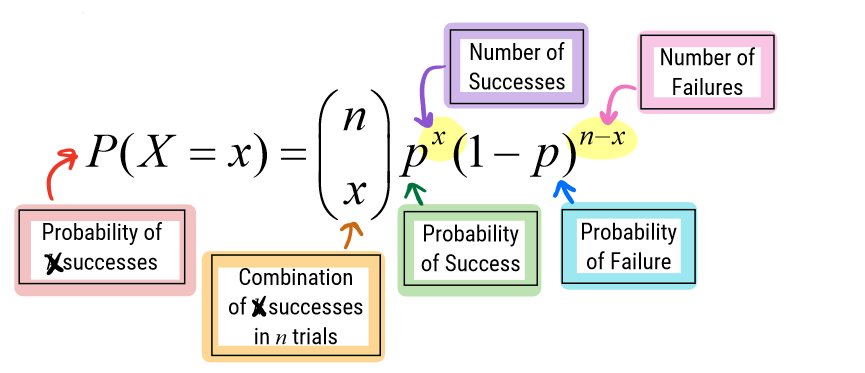
\includegraphics[width=0.8\textwidth]{4.7.1.PNG}
\end{center}

\begin{example}
    Explain how each of the following situations folows the binomial probability distribution model.

    (a) You toss a coin 10 times and count the number of tails you get.

    $X$ is the number of tails.
    \begin{itemize}
        \item Binary: Tails/Heads 
        \item Independence: Coin flips are independent
        \item Number of Trials: 10
        \item Probability: 0.50
    \end{itemize}

    Find and interpret P(X=4).

    $P(X=4)=\binom{10}{4}(0.50)^4(0.50)^{10-4}=0.2051$. The probability you get 4 tails in 10 coin flips is 20.51\%.

    (b) Type A blood is found in 43\% of the population. You have a group of 40 students.

    $X$ is the number of students with Type A blood.
    \begin{itemize}
        \item Binary: Type A/Not Type A 
        \item Independence: Assume many students in population 
        \item Number of Trials: 40
        \item Probability: 0.43
    \end{itemize}

    Find and interpret P(X=15)

    $P(X=15)=\binom{40}{15}(0.43)^{15}(0.57)^{25}=0.1008$. The probability you get 15 students out of 40 who have Type A blood is 10.08\%.
\end{example}

Distributions in your calculator often have ``pdf'' and ``cdf'' after them and there is an important difference.
\begin{itemize}
    \item pdf = probability distribution function and is used when you are trying to calculate $P(X=k)$
    \item cdf = cumulative distribution function and is used when you are trying to calculate $P(X\leq k)$
\end{itemize}

Specifically for binomial distributions, we want
\begin{itemize}
    \item 2nd - VARS - A:binompdf(trials, probability of success) for $P(X=k)$
    \item 2nd - VARS - B:binomcdf(trials, probability of success) for $P(X\leq k)$
\end{itemize}
A binomial random variable is discrete so how you set up your inequality matters.

\begin{example}
    Let $X$ = number of students that pass the AP Statistics Exam out of a class of 20. THe probability that a random student will pass is 0.62. Find the probability that 

    (a) All students pass hte exam.

    P(x=20) = binompdf(trials: 20, p: 0.62, x: 20) = 0.0007

    (b) Six or fewer students pass hte exam 

    P(x$\leq 6$) = binomcdf(trials:20, p: 0.62, x:6) = 0.0037

    (c) At least 12 students pass the exam 

    P(x$\geq 12$) = 1-P(x$\leq 11$) = 1 - binomcdf(trials:20, p:0.62, x:11) = 0.6659
\end{example}

\begin{example}
    Suppose the probability that any random freshman girl will agree to try out for a high school dance team is 10\% and one of the team captains asks 25 random freshman girls to try out.

    (a) What is the probability that exactly 1 will say yes?

    P($x=1$) = binompdf(trials: 25, p: 0.10, x: 1) = 0.1994

    (b) What is the probability that at least 1 will say yes?

    P($x\geq 1$) = 1 - P($x=0$) = 1 - binompdf(trials: 25, p: 0.10, x: 0) = 0.9282

    (c) On average, how many freshman girls will agree to try out for the team? Interpret in context.

    mean = $np$ = 2.5 girls. On average, if we select many groups of 25 freshman girls, we would expect 2.5 girls to try out.

    (d) What is the standard deviation of this binomial distribution? Interpret in context.

    $\sigma_x = \sqrt{np(1-p)}$ = 1.5 girls. The number of girls who try out typically differs from the mean by 1.5 girls.
\end{example}

\section{The Geometric Distribution}
When we perform many independent trials of the same chance process and are interested in the occurrence of the first success, a geometric setting arises.

Before attempting to calculate a geometric setting, check to make sure all of the following conditions have been met.

\begin{itemize}
    \item Binary - the possible outcomes can be classified as a success or failure 
    \item Independent - trials must be independent (the result of one trial tells us nothing about the result of another trial)
    \item First - you are interested in the number of trials until the first success.
    \item Success - the probability of success remains consistent trial to trial 
\end{itemize}

\begin{example}
    You roll a six-sided fair die. Let $X$ = number of trials until you roll a six. Complete the probability distribution table below.

    \begin{center}
        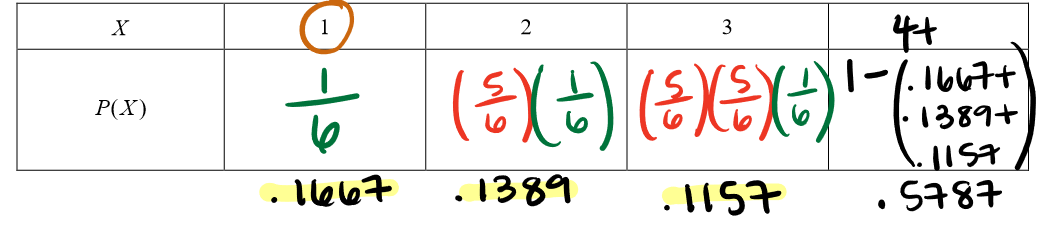
\includegraphics[width=0.8\textwidth]{4.8.1.PNG}
    \end{center}
\end{example}

If $X$ has a geometric distribution with a probability of success $p$ on each trial and $x$ represents the trial that you get your first success. The probability that $X$ equals $x$ is given by 
\[ P(X=x)=(1-p)^{x-1}(p) \]
Where $P(X=x)$ is the probability of first success on $x$ trial, $(1-p)$ is the probability of failure, $p$ is the probability of success, and $x-1$ is the number of failures.

\begin{example}
    You roll a six-sided fair die. Let $X$ = number of trials until you roll a six.

    (a) What is the probability that you get your first six on the 5th roll?

    P($X=5$) = $\left(\frac{5}{6}\right)^4\left(\frac{1}{6}\right) = 0.0804$

    (b) What is the probability that you get your first six within 3 rolls?

    P($X\leq 3$) = $P(X=1)+P(X=2)+P(X=3) = 0.1667+0.1389+0.1157 = 0.4213$.

    (c) What is the probability that it takes at least 4 rolls to get your first six?

    $P(X\geq 4)=1-P(X\leq 3) = 1-0.4213 = 0.5787$.
\end{example}

Specifically for geometric distributions, we want 
\begin{itemize}
    \item 2nd - VARS - E:geometpdf(probability of success, $k$) for $P(X=x)$
    \item 2nd - VARS - F:geometcdf(probability of success, $k$) for $P(X\leq x)$
\end{itemize}

Note: Your calculator can only do less than or equal to so all inequalities must be written in this manner.

\begin{example}
    Let $X$ = number of basket attempts needed for a college basketball player to make his first free throw. The player has an 82\% chance of making a random free throw. Find the probability that 

    (a) He makes his first basket on his fifth atempt.

    $P(X=5)$ = geometpdf(p = 0.82, x = 5) = 0.0009

    (b) It takes less than 4 attempts to make his first basket.

    $P(X<4)$ = geometcdf(p = 0.82, x: 3) = 0.9942

    (c) It takes at least 3 attempts to make his first basket.

    $P(X\geq 3) = 1-P(X\leq 2) =$ 1 - geometcdf(p: 0.82, x: 2) = 0.0324

    (d) He will make 6 baskets in a row before he misses.

    $P(X=7)=(0.82)^6(0.18)$= geometpdf(p: 0.18, x: 7) = 0.0547
\end{example}

Like all probability distributions, the geometric distribution has a mean and a standard deviation. If $X~G(p)$ then: 
\[ \mu_x = \frac{1}{p}\]
\[ \sigma_x = \frac{\sqrt{1-p}}{p} \]

\begin{example}
    Drew decides to place a \$10 bet on Number 3 in consecutive spins of a roulette wheel until he wins. On any spin, Drew has a 1/38 chance that the ball will land in the Number 3 slot. Let $X$ = number of spins until first win.

    (a) How many spins do you expect it to take until Drew wins? What does this typically vary by?

    $\mu_x = \frac{1}{1/38}$ = 38 spins.

    $\sigma_x = \frac{\sqrt{1-\frac{1}{38}}}{\frac{1}{38}}=37.4967$ spins 

    Recall: if an event has a probability less than 5\%, we consider it to be rare/unusual/surprising if it were to actually happen.

    (b) Would you be surprised if it took 10 or fewer spins for Drew to win? Calculate a probability to support your answer.

    $P(X\leq 10)$ = geometcdf(p: $\frac{1}{38}$, x: 10) = 0.2341, non unusual.

    The probability of this occurring is approximately 23.41\%, so it would not be surprising.

    (c) Would you be surprised if it took more than 13 spins of roulette wheel until he won? Calculate a probability to support your answer.

    $P(X>13) = 1-P(X\leq 13) = 1-$geometcdf(p: $\frac{1}{38}$, x: 13) = 0.7070.

    The probability of this occurring is approximately 70.70\%, so it would not be surprising.
\end{example}
\end{document}
